\subsection{Zustandsbeobachter}
    Lineare Zustandsregler (wie z.B. LQR) basieren auf der Kentniss von $x(t)$. Das ist praktisch aber nicht umsetzbar. Deshalb benutzt man \emph{Zustandsbeobachter} um durch $u(t)$ und $y(t)$ eine Schätzung $\widehat{x}(t)$ zu erhalten.
    
    \subsection{Luenberger Beobachter}
        Man will eine Beobachterdynamik $\frac{d}{dt}\widehat{x}(t)$ s.t. der Beobachtungsfehler $e(t) = x(t) - \widehat{x}(t)$ asymptotisch zu Null konvergiert $\displaystyle\lim_{t\to\infty}e(t) = 0$.
        
        \begin{align*}
            \frac{d}{dt}\widehat{x}(t) &= \widehat{A}\cdot\widehat{x}(t)+\widehat{B}\cdot u(t) + L\cdot\big(y(t)-\widehat{y}(t)\big)\\
            \widehat{y}(t) &= \widehat{C}\cdot\widehat{x}(t)
        \end{align*}
        
        \begin{figure}[H]
            \centering
            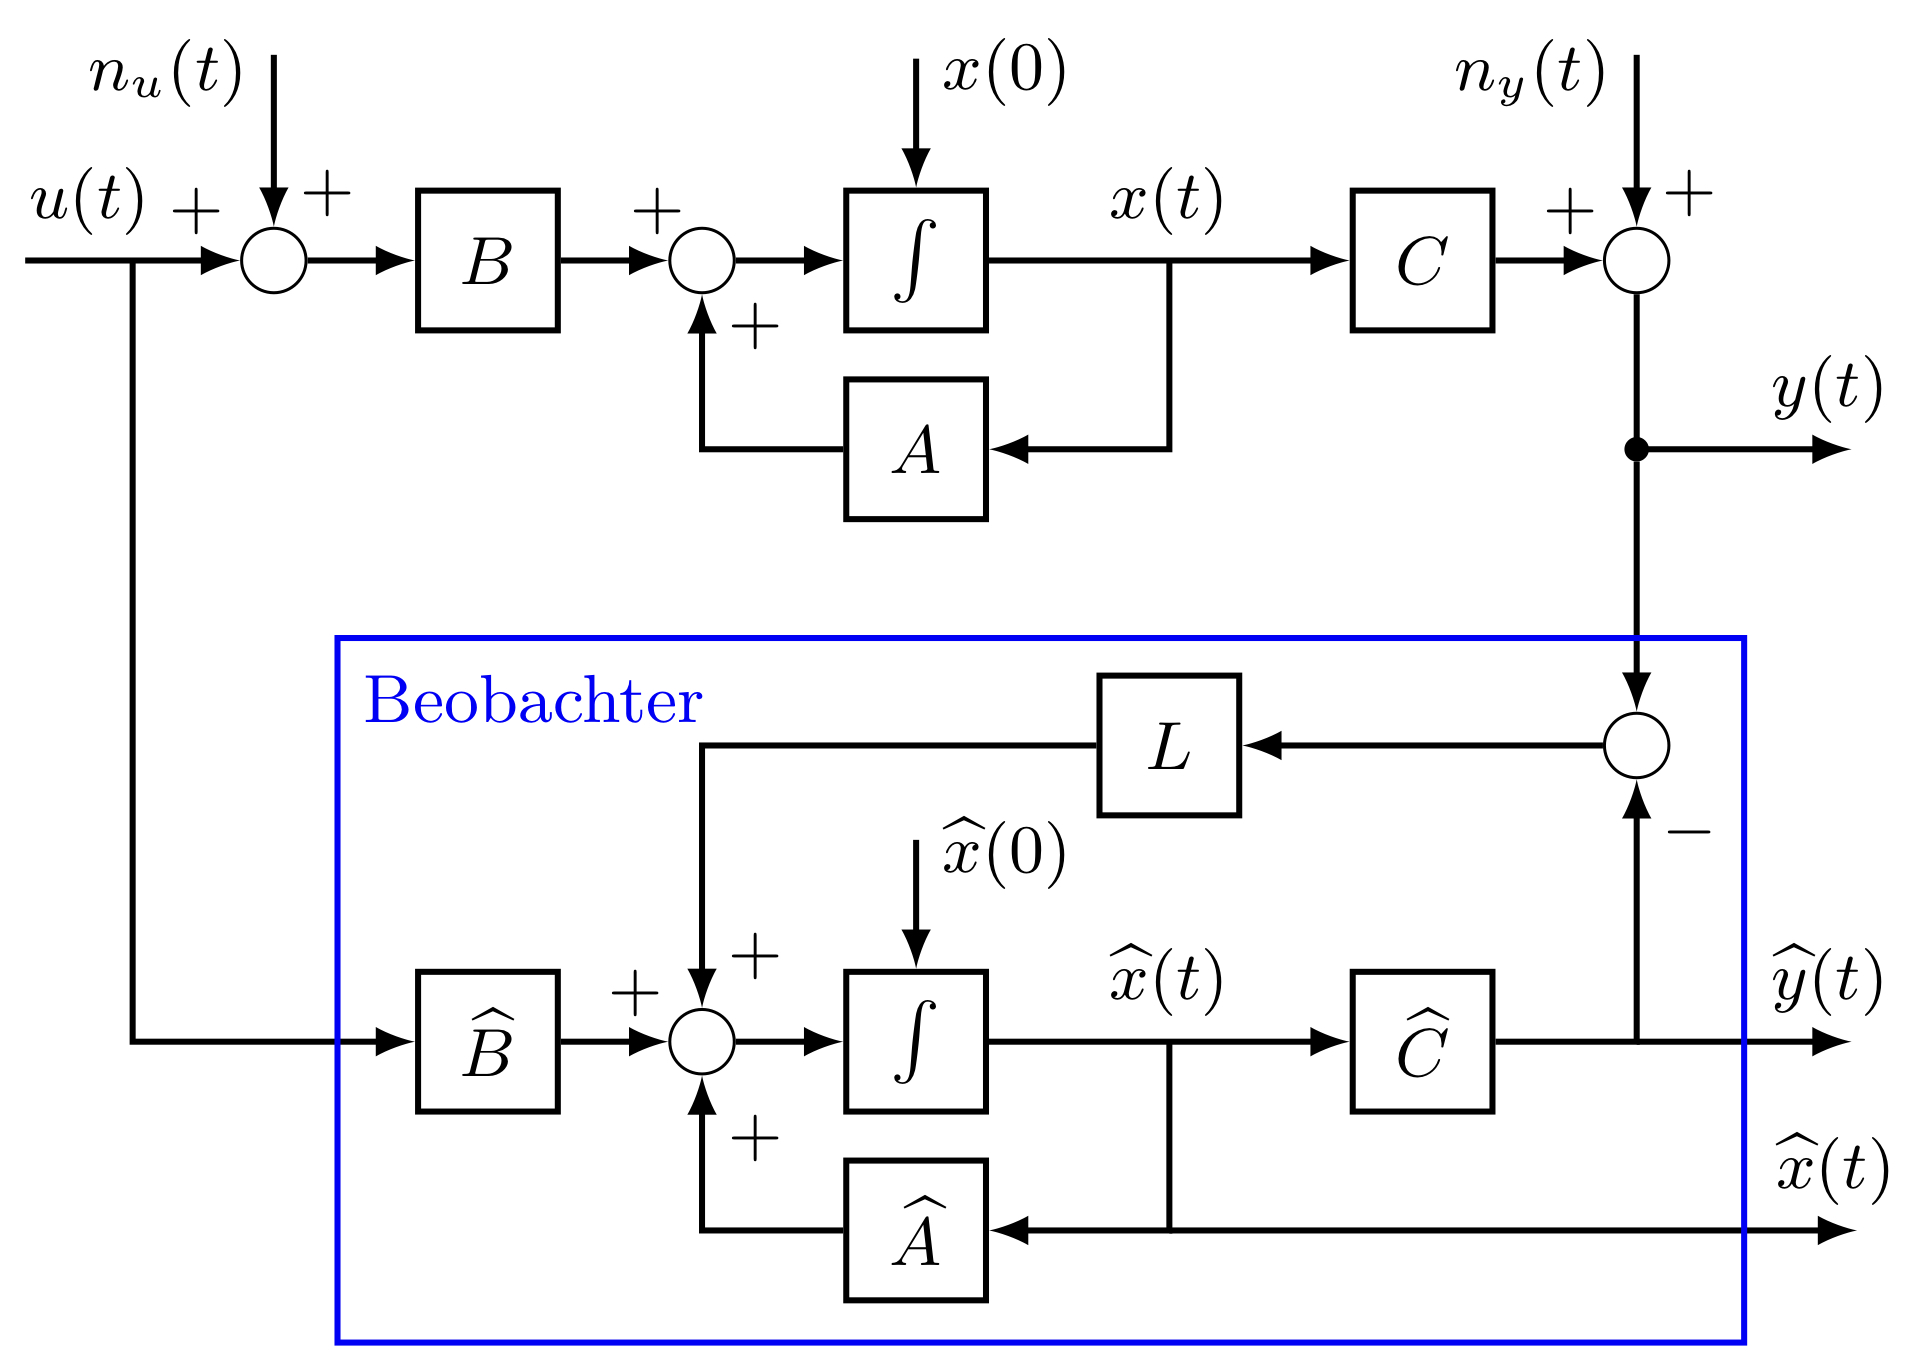
\includegraphics[width = 0.7\linewidth]{images/09/luenberger_obsv.jpeg}
            \caption{Blockdiagramm des Luenberger Observeres}
        \end{figure}
        
        Unter der Annahme, dass ein perfektes Modell vorliegt \big(i.e. $\widehat{(\cdot)} = (\cdot)$\big) ergibt sich Folgende Fehlerdynamik:
        \begin{equation*}
            \colorboxed{red}{\frac{d}{dt}e(t) = \big(A- L\cdot C\big)\cdot e(t)},\quad e(0) = x(0)-\widehat{x}(0) \neq 0
        \end{equation*}
        Fehler konvergiert zu 0 falls $A- L\cdot C$ Hurwitz ist. Dies kann unter anderem durch zwei Arten erreichen:
             
        \subsubsection{Pole Placement}     
             Man platziert die gewünschten Polynome von Hand indem man $L$ durch folgende Gleichung bestimmt:
            \begin{equation*}
                \det\big(A-L\cdot C - \lambda I) \overset{!}{=} (\lambda_1 - \lambda)(\lambda_2 - \lambda)\dots(\lambda_n - \lambda) = 0
            \end{equation*}
            Dabei sind $\lambda_i$ die gewünschten EW. Die Einträge der Matrix $L$ folgen dann aus den Vergleichen mit den $\lambda_i$.
            
        \subsubsection{LQR Formulierung}
            Da die $L$ und $C$ Matrizen ``vertauscht'' sind für die LQR Formulierung und da gilt
            \begin{equation*}
                \operatorname{eig}(X) = \operatorname{eig}(X^\top),\quad X\in\mathbb{R}^{n\times n}
            \end{equation*}
            können wir mit LQR Formulierung für die Matrix $A^\top - C^\top\cdot L^\top$ die Matrix $L$ bestimmen, welche uns die MAtrix $A-L\cdot C$ Hurwitz macht.
            
            Mit den Änderungen
            \begin{align*}
                A&\rightarrow A^\top, & B&\rightarrow C^\top\\
                Q = \Bar{C}^\top\cdot\Bar{C}&\rightarrow \Bar{B}\cdot\Bar{B}^\top & R= r\cdot I &\rightarrow q\cdot I\\
                K &\rightarrow L^\top & \Phi &\rightarrow \Psi
            \end{align*}
            foglt für die Lösung der LQR Formulierung:
            \begin{equation*}
            \colorboxed{red}{
            \begin{aligned}
                &L^\top = \frac{1}{q}\cdot C\cdot \Psi\\
                &\Psi \cdot C^\top\cdot\frac{1}{q}\cdot C\cdot \Psi-\Psi\cdot A^\top-A\cdot\Psi-\Bar{B}\cdot\Bar{B}^\top = 0
            \end{aligned}
            }
            \end{equation*}
            
            Falls die Matrizen $\{A,C\}$ beobachtbar und $\{A,\Bar{B}\}$ steuerbar sind, existiert eine eindeutige positiv definite Lösung $\Psi$.
            
            \textbf{Bemerkungen:}
            \begin{itemize}
                \item $L$ ist statisch (muss nur einaml berechnet werden)
                \item Matrizen $\Bar{B}$ und $q$ werden iterativ getunt bis Resultat zufriedenstelligend ist.
                \item Falls $n_y\neq0$ ist $\frac{d}{dt}e(t)$ noch um $-L\cdot n_y(t)$ erweitert. $L$ kann nicht beliebig gross gewählt werden.
            \end{itemize}
            
            \begin{figure}[H]
                \centering
                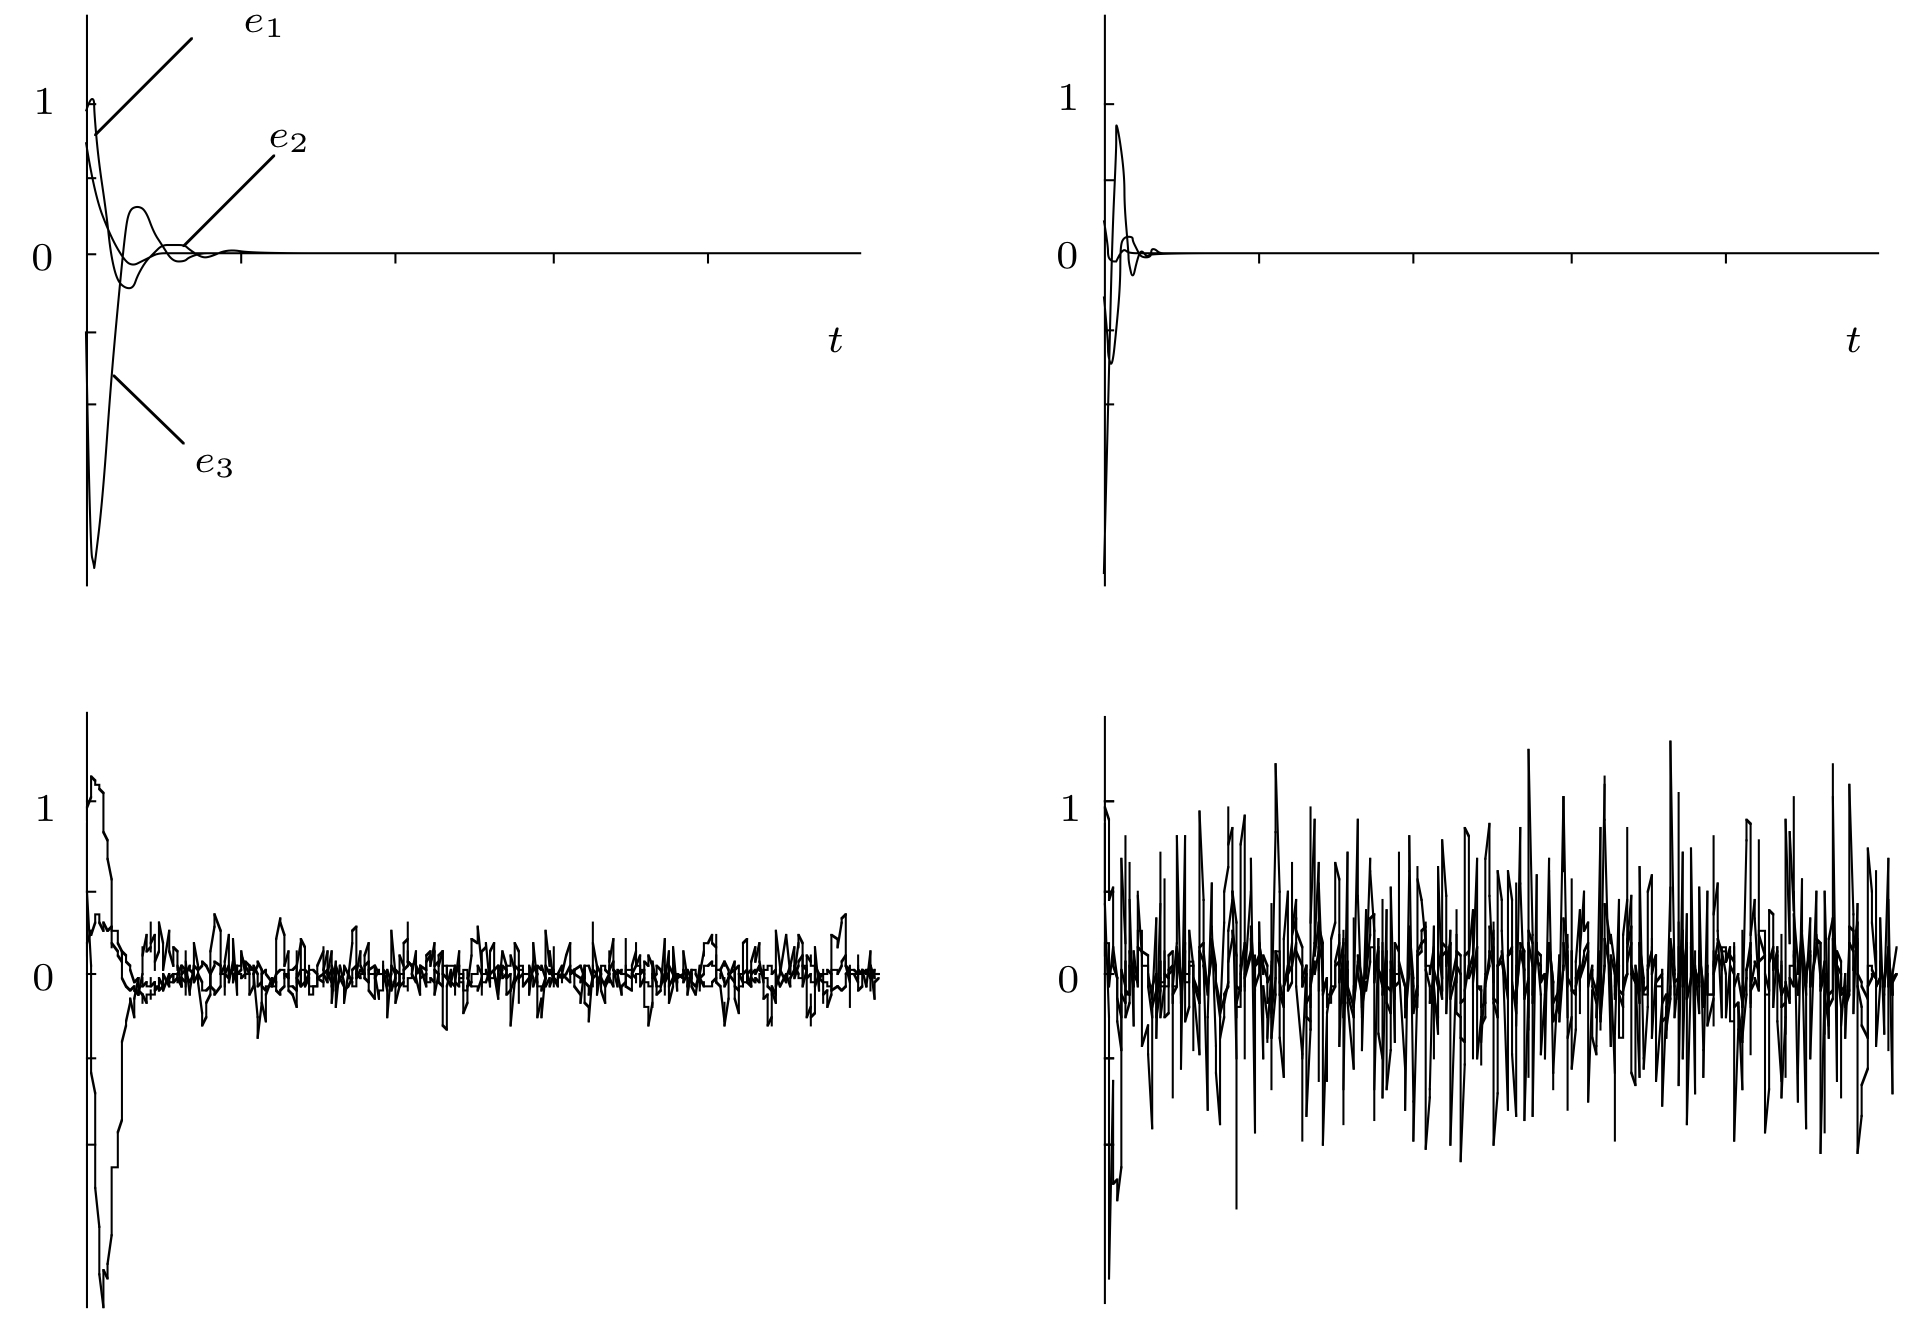
\includegraphics[width = 0.7\linewidth]{images/09/L_noise.jpeg}
                \caption{Links ``Langsames" $L$, Rechts ``schnelles" $L$}
            \end{figure}